\section{Hierarchical clustering with Dummy variables}

% \begin{itemize}
%     \item Present the results of the hierarchical clustering analysis. This include dendrogram plots, cluster sizes, and statistics.
%     \item Describe the number of clusters or groups identified and their characteristics.
%     \item Provide profiles or descriptions of the clusters. Discuss what makes each cluster unique in terms of viewing patterns and behavior.\\
%     Include statistics or visualizations that highlight the key features of each cluster.
%     \item Recommendations for the Recommender System.\\
%     Explain how the clustering results can be applied to the recommender system.\\
%     Describe how content recommendations can be tailored to each cluster's preferences.\\
%     Discuss any challenges or considerations in implementing these recommendations.
%     \item Evaluation of the Recommender System\\
%     Discuss how the clustering-based recommender system was evaluated, including metrics such as accuracy, user satisfaction, or engagement.\\
%     Present the results of the evaluation and any improvements made based on feedback.
%     \item Pros and Cons of methods using to analysis
% \end{itemize}



\subsection{Problem}
    Regarding the objective of the project, users with similar viewing patterns need to be grouped together in a cluster, and in the previous section, we know that the dataset consists of both numerical and categorical data. Especially, it is impossible to calculate the distance between any 2 entries of the data frame by applying mathematical algorithms (Euclidean, Manhattan, Canberra, etc) directly since all variables are not numerical. To handle this situation, an encode is needed to convert variables from nominal to numerical type. (The conversion from ordinal variables to numerical variables is redundant since ordinal variables could be labeled with levels and then be scaled to behavior as numerical variables). That encoding is called \textbf{\textit{Dummy variables}}, and this section will discuss the implementation of dummy variables for hierarchical clustering.

\subsection{Dummy variables}

        \begin{itemize}
            \item \textbf{\underline{Definition:}} A Dummy (or Indicator) variable is an artificial variable created to represent a categorical variable with two or more distinct categories or levels.

            \item \textbf{\underline{Usage:}} With dummy variables, all nominal variables could be converted to numerical. Hence, it is possible to apply mathematical algorithms to start the analysis process.

            \item \textbf{\underline{Example:}} A nominal variable named "Genre" always takes one of 3 values "Action", "Comedy", and "Fantasy". After converting it into the dummy variable: 
            \begin{itemize}
                \item[-] If the value of the variable is "Action", the indicator for "Genre.Action" attribute will be 1, and other attributes are 0's.
                \item[-] If the value of the variable is "Comedy", the indicator for "Genre.Comedy" attribute will be 1, and other attributes are 0's.
                \item[-] If the value of the variable is "Fantasy", the indicators for all attributes are 0's.
            \end{itemize}
            
        \end{itemize}

\begin{table}[h]
\centering
 \begin{subtable}[b]{0.45\linewidth}
    \centering
      \begin{tabular}{|l|}
        \hline
          \cellcolor{blue!25}Genre \\
        \hline
         Action \\
         \hline
         Comedy \\
         \hline
          Fantasy \\
          \hline
       \end{tabular}
       \caption{Original "Genre" variable}
    \end{subtable}%
 \begin{subtable}[b]{0.45\linewidth}
        \centering
        \begin{tabular}{|l|c|c|}
            \hline
             & Genre.Action & Genre.Comedy \\
            \hline
            Action & 1 & 0 \\
            \hline
            Comedy & 0 & 1 \\
            \hline
            Fantasy & 0 & 0 \\
            \hline
        \end{tabular}
        \caption{"Genre" Dummy variable}
    \end{subtable}
    \caption{Using Dummy variables}
\end{table}

$\rightarrow $ A variable which has a total of $n$ different values will have new $n - 1$ attributes after converting to a dummy variable, and the last value has the indicators for all attributes are 0's.


\subsection{Applying the Hierarchical clustering model}

    \begin{itemize}
        \item In this section, R programming language is used as the main language to implement the hierarchical clustering model.

         \item Dependencies (List of packages used):

                 \begingroup
                    \setlength{\tabcolsep}{10pt} % Default value: 6pt
                    \renewcommand{\arraystretch}{1.2} % Default value: 1
                    \begin{tabular}{ | l | l |  l |} % l for left, c for center
                      \hline
                    \textbf{Package name} & \textbf{Description} & \textbf{Version} \\
                      \hline 
                    base & The R Base Package & $\ge 4.3.2$\\
                      \hline
                    cluster & Finding Groups in Data &  $\ge 2.1.4 $ \\
                      \hline
                    factoextra & clustering visualization &  $\ge 1.0.7 $ \\
                      \hline
                    gplots & plotting data, dendrogram &  $\ge 3.1.3 $ \\
                      \hline
                    ggplot2 & draw distribution graph &  $\ge 3.4.4 $ \\
                      \hline
                      
                    \end{tabular}
                \endgroup
         
    \end{itemize}

   
    \vspace{2mm}
    
    (Source code link: \url{https://github.com/vhtuananh020402/Group4_Data_analysis/blob/main/dummy_canberra_ward.r})
    
    \vspace{2mm}

    To start applying the hierarchical clustering model, first, the dataset is imported and stored as a data frame in R. The function \textbf{\textit{na.omit()}} is necessary for omitting the missing value of the imported data frame. 
    \begin{code}{R}
        # Read the data frame
        df <- read.csv("data/clean_data_v2.csv")
        
        # Omit the NA values of the data frame
        df <- na.omit(df)
    \end{code}

    Then, we standardize (scale) the "Age" (numerical) variables. Since the "Frequency" variable is ordinal, it first needs to be ordered and labeled with levels, then converted to a numerical variable using \textbf{\textit{as.numeric()}} function. After that, the "Frequency" (numerical) variable is scaled.

    \begin{code}{R}
        # Standardize the Age variable
        df$Age_std <- scale(df$Age)
        
        # Standardize the Frequency variable
        df$Frequency <- factor(
              df$Frequency, 
              order = TRUE,
              levels = c("Less than 2 hours", "2 - 5 hours", "6 - 10 hours", "11 - 15 hours", "16 - 20 hours", "More than 20 hours"))
        df$Frequency_numeric <- as.numeric(factor(df$Frequency))
        df$Frequency_std <- scale(df$Frequency_numeric)
    \end{code}

    The function \textbf{\textit{model.matrix()}} is used to create a data frame matrix consisting of all numerical variables (all nominal variables "Genre", "Field", "Factor", "Gender", "Platform" are converted to dummy variables)
    
    \begin{code}{R}
        # Turn the nominal variables into dummy variables
        df_dummy <- model.matrix(~ Age_std + Genre + Frequency_std + Field + Factor + Gender + Platform, data = df)
    \end{code}

    Here we use Canberra algorithms to calculate the points distance and Ward's method to calculate the clusters distance. Then we can visualize the hierarchical clusters by using the function \textbf{\textit{plot()}} to plot a dendrogram.
    
    \begin{code}{R}
        # Calculate the points distance
        point_dist <- dist(df_dummy, method = "canberra")      # Using Canberra distance
        
        # Hierarchical cluster analysis on the data frame
        hc <- hclust(point_dist, method = "ward.D")            # Using Ward's method
        
        # Plot the dendrogram
        dend <- as.dendrogram(hc)
        plot(dend)
    \end{code}

    \begin{figure}[H]
        \centering
        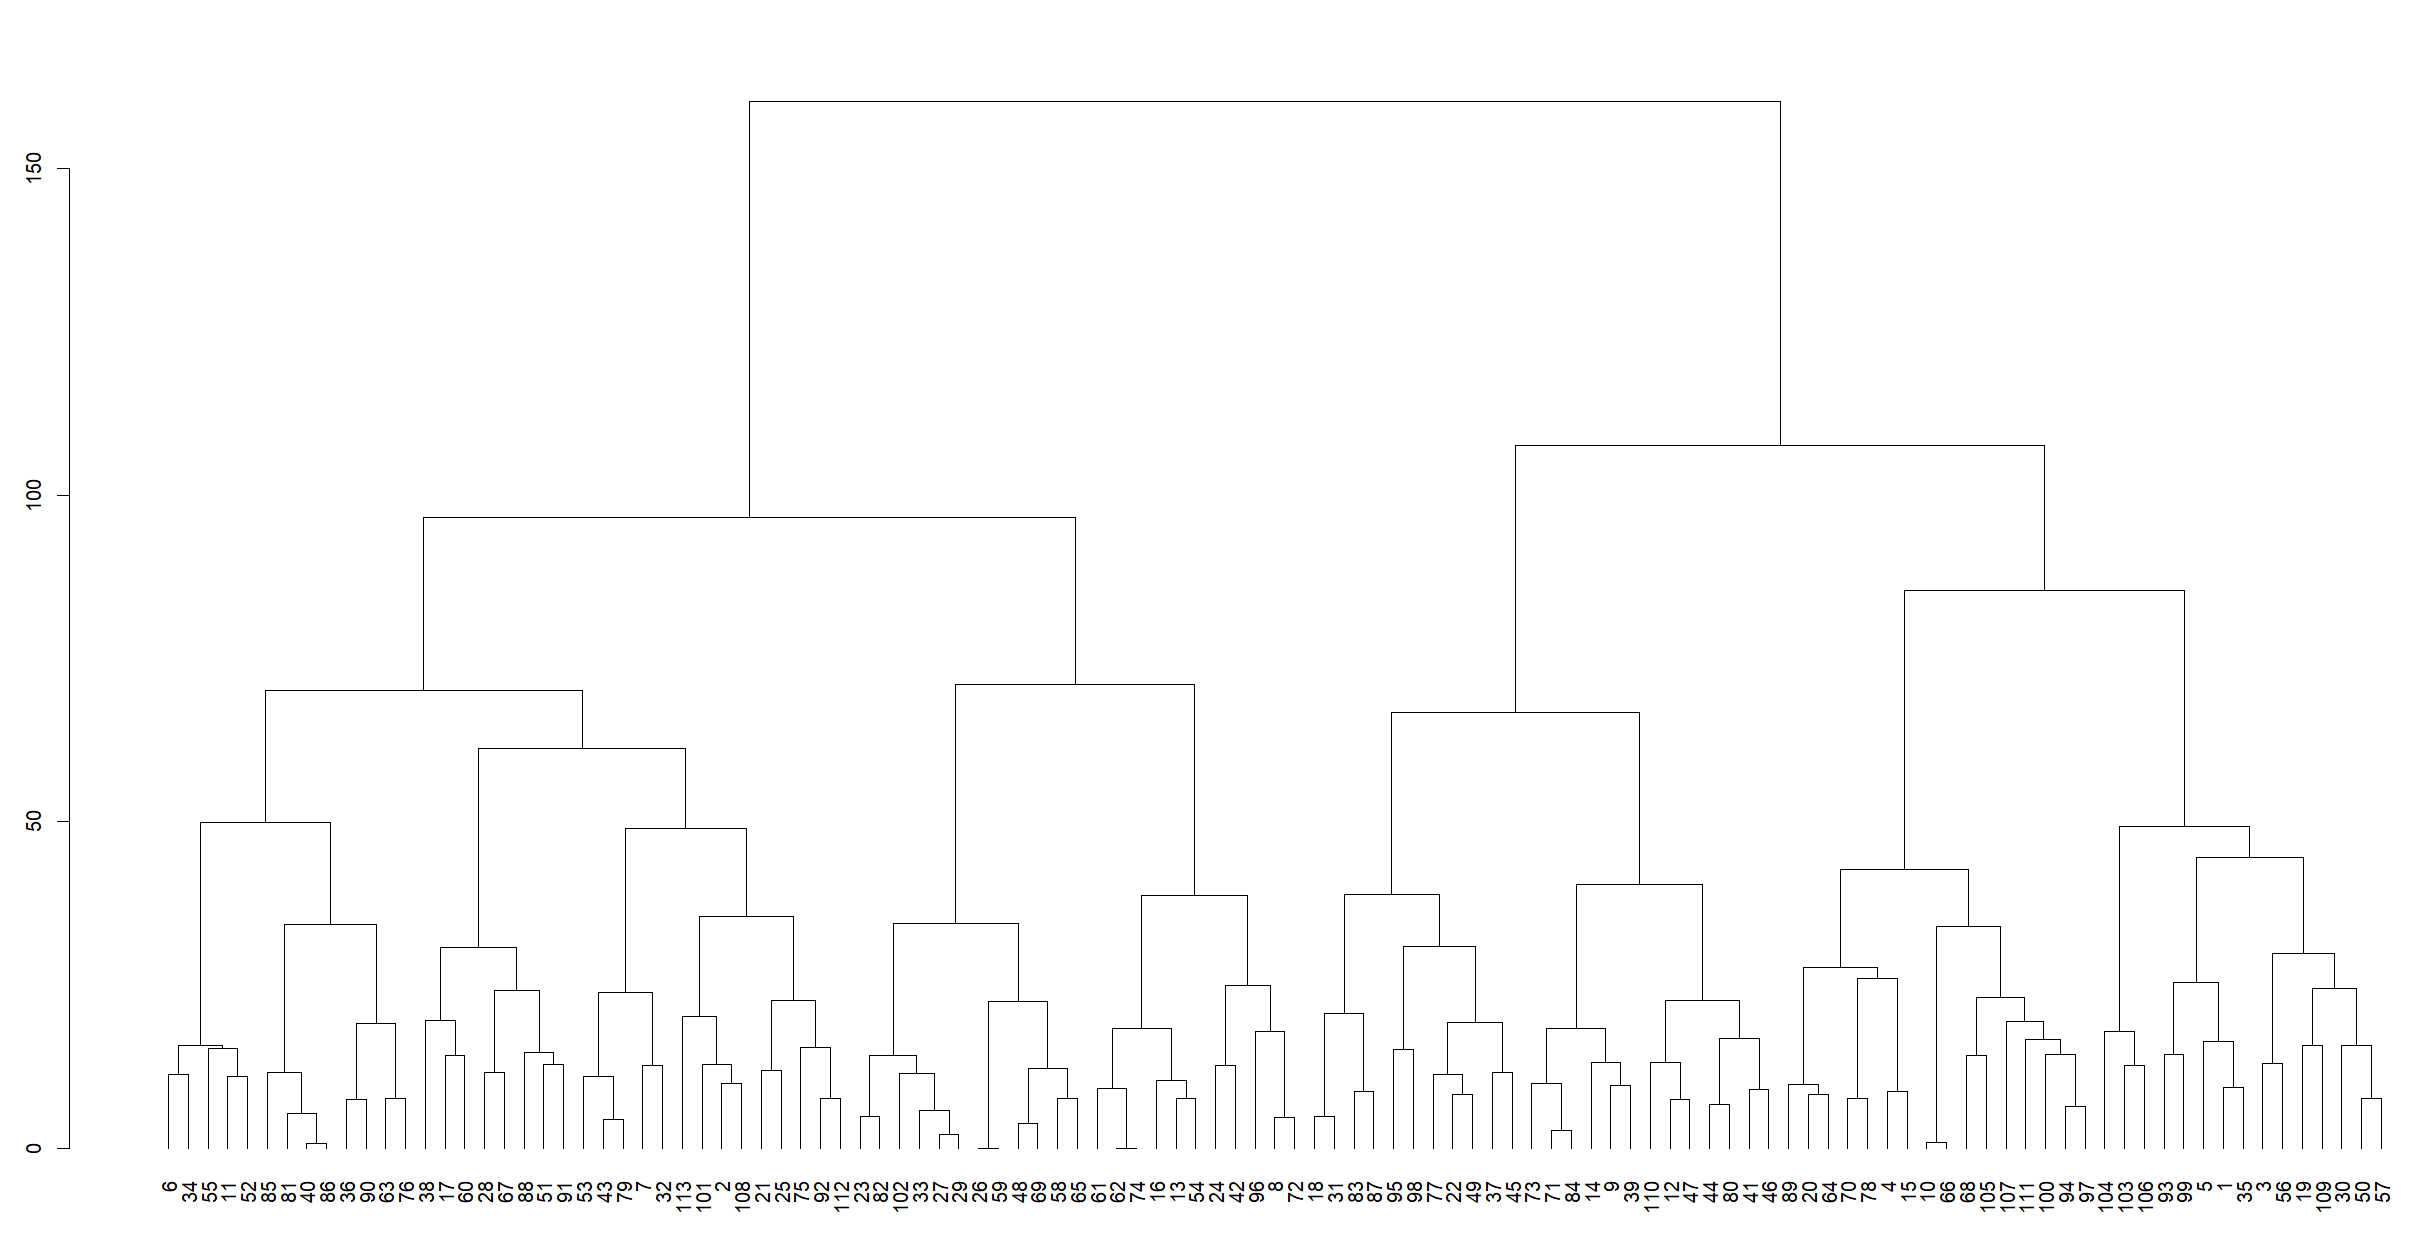
\includegraphics[scale=0.3]{graphics/dummy/dendrogram/dendrogram1.png}
        \caption{Dendrogram visualization }
    \end{figure} 

\subsection{Finding the optimal number of clusters}
 After dendrogram visualization, as can be clearly seen that there are many possible numbers of clusters to choose from for analysis. Each different number of clusters will bring different outcomes, thus we need an exact optimal number of clusters, and there are some methods that help us to find it, \textbf{Gap Statistics} is one of the most well-known and easily understandable methods to find the optimal number of clusters, so this section will focus on it.
 
    \subsubsection{Gap statistics method}

    \begin{itemize}
        \item This approach can be applied to any clustering method.

        \item The estimate of the optimal clusters will be the value that maximizes the gap statistic. This means that the clustering structure is far away from the random uniform distribution of points.

        \item R code implementation:
    \end{itemize}

    \begin{code}{R}
        # ======= Gap statistic method to find the optimal number of cluster  =======
        # Calculate Within-Cluster Dispersion (WCD) for the original data
        wss <- sum(hc$height)
        
        # Generate Random Data for Comparison
        set.seed(123)   # Set seed for reproducibility
        B <- 100        # Number of random datasets
        random_datasets <- lapply(1:B, function(i) matrix(runif(length(df_dummy)), ncol = ncol(df_dummy)))
        
        # Cluster the Random Data
        random_hcs <- lapply(random_datasets, function(random_data) {
          dist_matrix <- dist(random_data, method = dist_method[4])
          hclust(dist_matrix, method = hc_method[1])
        })
        
        # Calculate Within-Cluster Dispersion for Random Data
        wss_random <- sapply(random_hcs, function(random_hc) sum(random_hc$height))
        
        # Calculate Gap Statistic    
        gap <- (log(wss_random) - log(wss)) + mean(log(wss_random) - log(wss))
        
        # Determine the Optimal Number of Clusters
        num_clusters <- 1 : 10 # Desired number of cluster domain
        gap <- gap[1:length(num_clusters)]   
        x_labels <- seq(1, length(num_clusters))
        
        plot(num_clusters, gap, xlab = "Number of Clusters", ylab = "Gap Statistic", 
             main = "Gap Statistic Plot", type = "b")
        
        # Customize x-axis labels
        axis(1, at = x_labels, labels = num_clusters)
        abline(v = 8, col = "red", lty = 2)
    \end{code}


    \begin{figure}[H]
        \centering
        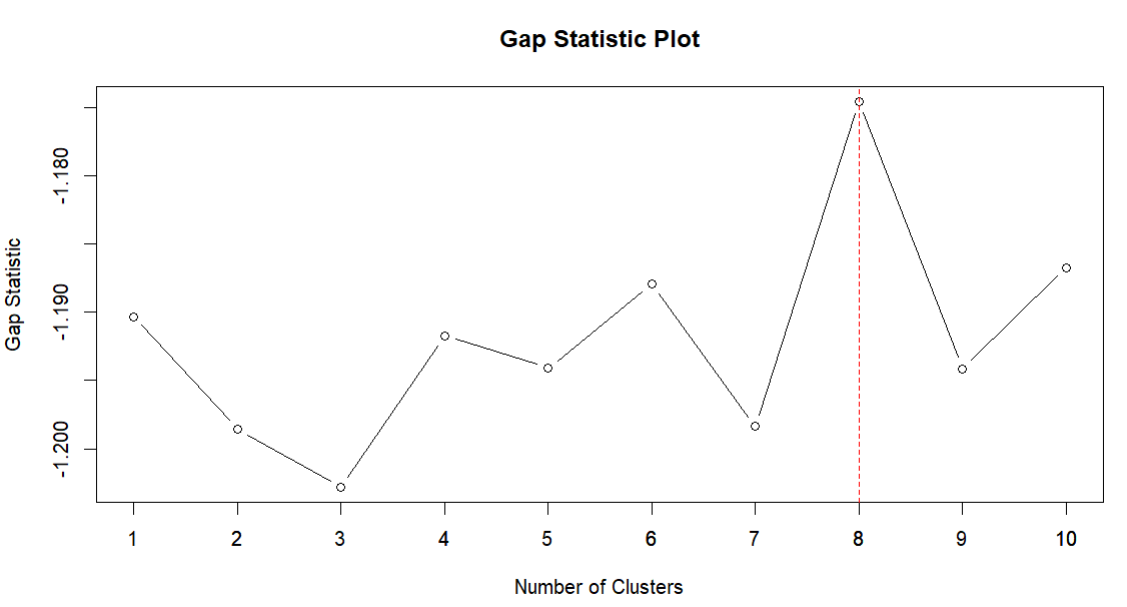
\includegraphics[scale=0.53]{graphics/dummy/gapStatistics/gapStatistics.png}
        \caption{Gap Statistics diagram}
    \end{figure}

    $\rightarrow$ From the above Gap Statistics diagram (range $1 : 10$), the highest point which indicates the optimal number of clusters for the dendrogram is 8. Hence, we chose the number 8 for the number of clusters for the dendrogram. 
    

\subsection{Result}
    \subsubsection{Dendrogram}


    \begin{code}{R}
        # Draw the rectangle around each cluster in k clusters
        k <- 8
        rect.hclust(hc, k, border = 2:8)
    \end{code}
    
    Here is the final dendrogram with 8 clusters, each cluster has a rectangle around it. The observations in each cluster have a close relationship, which will be discussed right after this dendrogram.

    \begin{figure}[H]
        \centering
            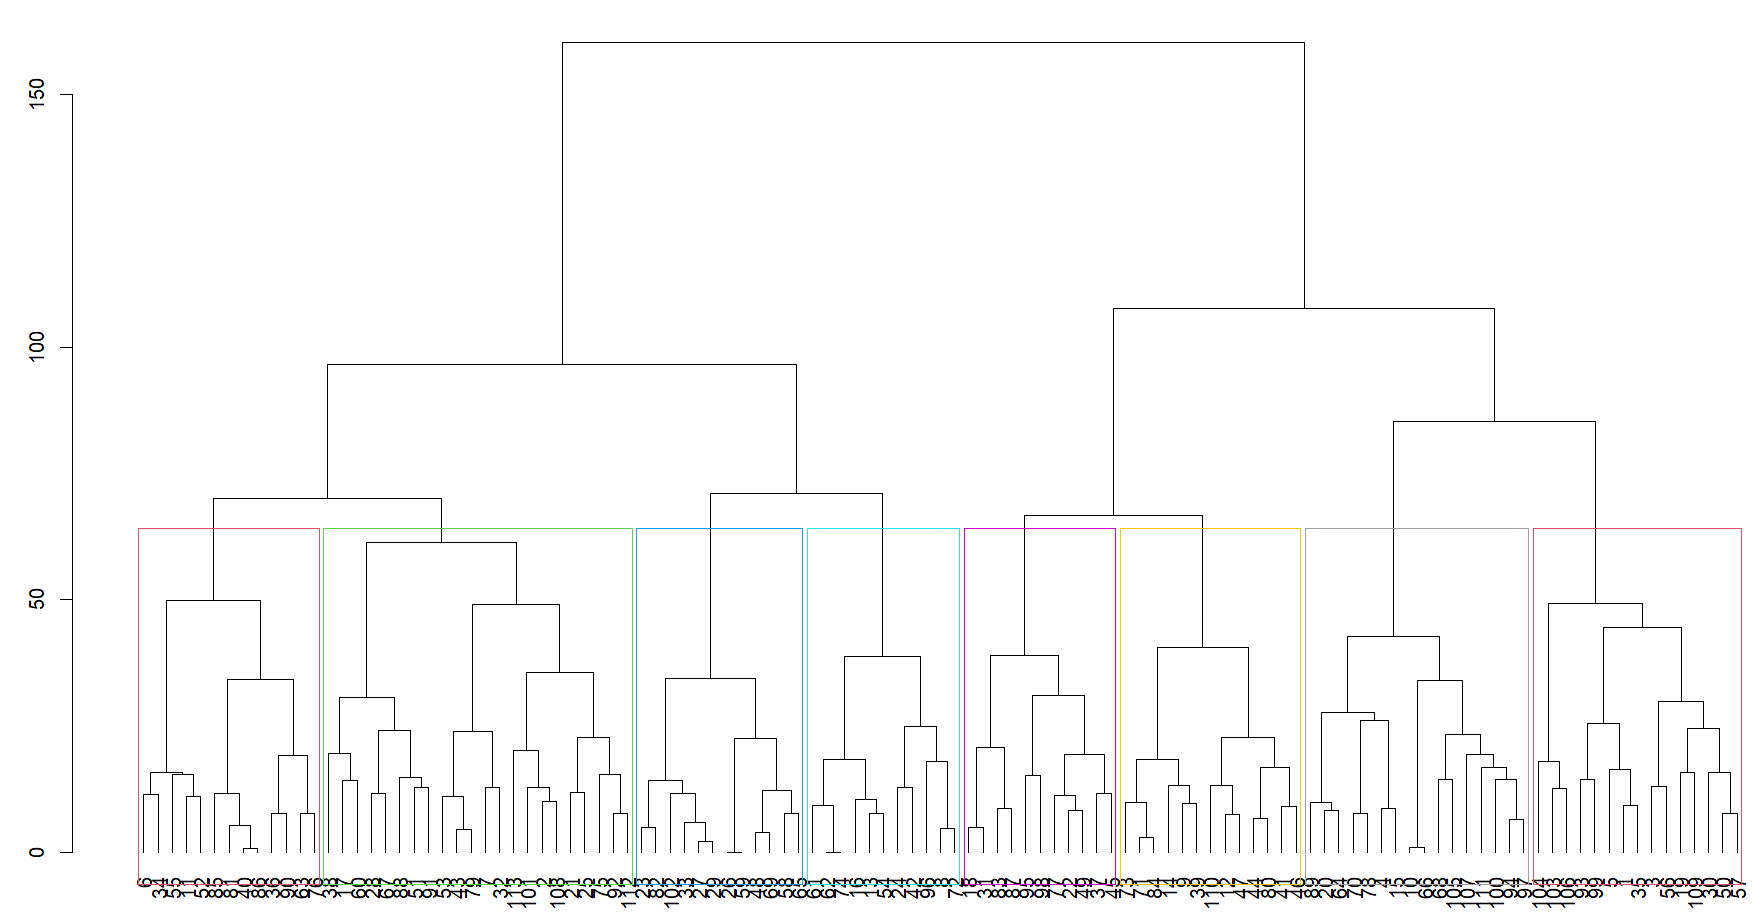
\includegraphics[scale=0.4]{graphics/dummy/dendrogram/dendrogram2.png}
        \caption{Age Distribution in each cluster}
    \end{figure}


    \subsubsection{Histogram and observing patterns}
 "Age", "Genre", "Field", "Frequency", and "Factor" are considered the main attributes of the movie genre recommender system, then we observe the patterns of those attributes by histograms.

 R code to plot the histograms for each cluster:
 \begin{code}{R}
    # Add the cluster assignments to the data frame
    df$Cluster <- factor(clusters)

    # Create a histogram of the Genre distribution in each cluster
    ggplot(df, aes(x = Genre)) +
      geom_histogram(stat = "count", fill = "lightblue", color = "black", linewidth = 0.8) +
      facet_wrap(~ Cluster) +
      theme(axis.text.x = element_text(angle = 45, hjust = 1)) +
      labs(title = "Genre Distribution in Each Cluster", x = "Genre", y = "Count")
    
    # Create a histogram of the Age distribution in each cluster
    ggplot(df, aes(x = Age)) +
      geom_histogram(stat = "count", fill = "orange", color = "black", linewidth = 0.8) +
      facet_wrap(~ Cluster) +
      theme(axis.text.x = element_text(angle = 45, hjust = 1)) +
      labs(title = "Age Distribution in Each Cluster", x = "Age", y = "Count")
    
    # Create a histogram of the Field distribution in each cluster
    ggplot(df, aes(x = Field)) +
      geom_histogram(stat = "count", fill = "red", color = "black", linewidth = 0.8) +
      facet_wrap(~ Cluster) +
      theme(axis.text.x = element_text(angle = 45, hjust = 1)) +
      labs(title = "Field Distribution in Each Cluster", x = "Field", y = "Count")
    
    # Create a histogram of the Frequency distribution in each cluster
    ggplot(df, aes(x = Frequency)) +
      geom_histogram(stat = "count", fill = "darkgrey", color = "black", linewidth = 0.8) +
      facet_wrap(~ Cluster) +
      theme(axis.text.x = element_text(angle = 45, hjust = 1)) +
      labs(title = "Frequency Distribution in Each Cluster", x = "Frequency", y = "Count")
    
    # Create a histogram of the Factor distribution in each cluster
    ggplot(df, aes(x = Factor)) +
      geom_histogram(stat = "count", fill = "lightgreen", color = "black", linewidth = 0.8) +
      facet_wrap(~ Cluster) +
      theme(axis.text.x = element_text(angle = 45, hjust = 1)) +
      labs(title = "Factor Distribution in Each Cluster", x = "Factor", y = "Count")
 \end{code}

    \begin{figure}[H]
        \centering
        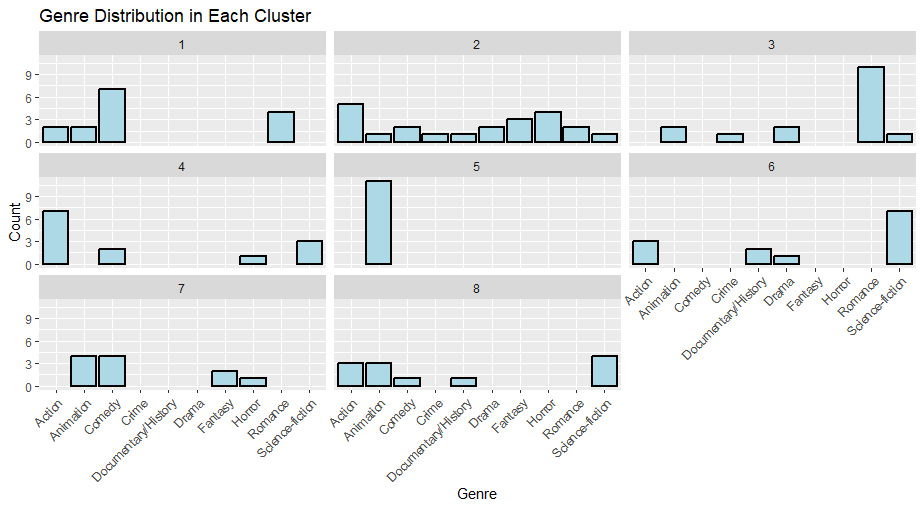
\includegraphics[scale=0.55]{graphics/dummy/distribution/GenreDistribution.png}
        \caption{Genre Distribution in each cluster}
    \end{figure}

    \begin{figure}[H]
        \centering
        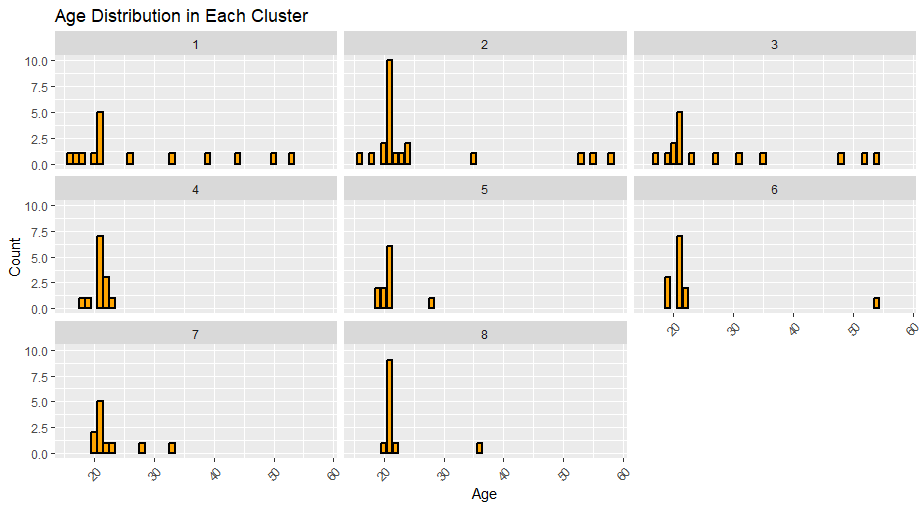
\includegraphics[scale=0.6]{graphics/dummy/distribution/AgeDistribution.png}
        \caption{Age Distribution in each cluster}
    \end{figure}

    \begin{figure}[H]
        \centering
        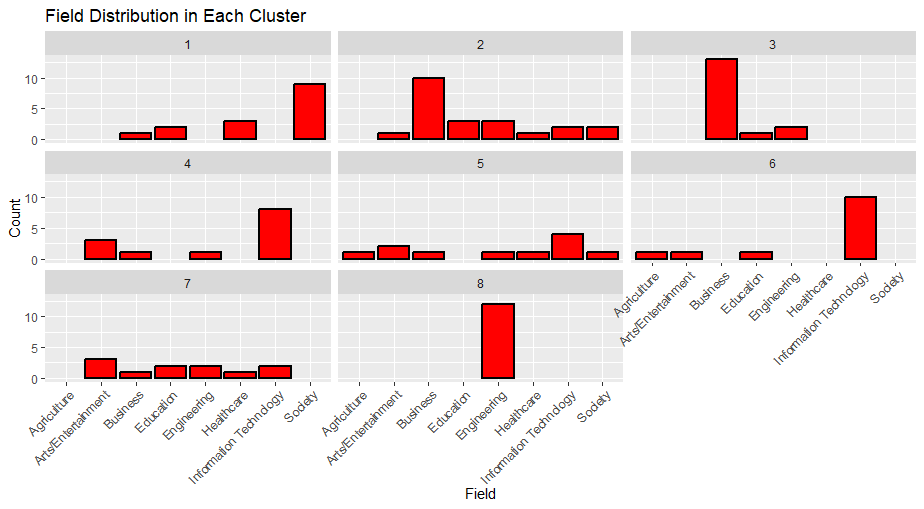
\includegraphics[scale=0.6]{graphics/dummy/distribution/FieldDistribution.png}
        \caption{Field Distribution in each cluster}
    \end{figure}

    \begin{figure}[H]
        \centering
        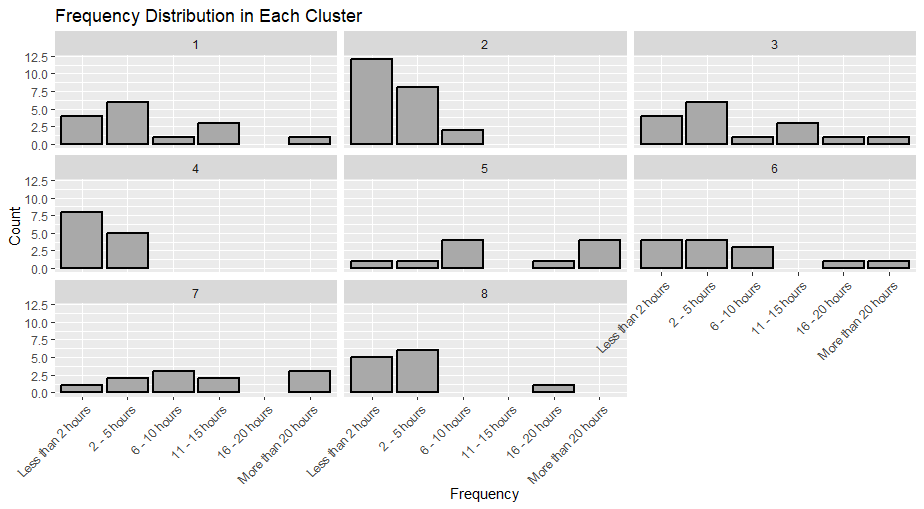
\includegraphics[scale=0.6]{graphics/dummy/distribution/FrequencyDistribution.png}
        \caption{Frequency Distribution in each cluster}
    \end{figure}

    \begin{figure}[H]
        \centering
        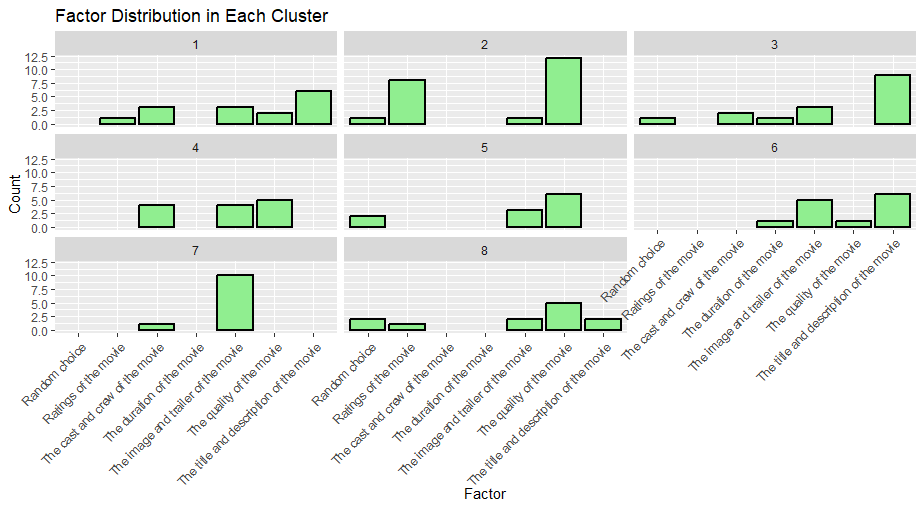
\includegraphics[scale=0.6]{graphics/dummy/distribution/FactorDistribution.png}
        \caption{Factor Distribution in each cluster}
    \end{figure}

From the histograms, here are conclusions for each cluster:

\begin{itemize}
    \item \textbf{\underline{Cluster 1:}} \textbf{Comedy} is the most favorite genre followed by \textbf{Romance}, with the majority of viewers being 21 years old and a small number ranged from 22 to 55 years old. Watching time is from 2 to 5 hours per week. Society field is the highest choice here. “Title/Description” is the most popular reason for choosing and watching.

    \item \textbf{\underline{Cluster 2:}} \textbf{Action}, \textbf{Horror}, and \textbf{Fantasy} are top-viewed genres (Romance and Drama are also considered). The viewers are mostly under 25 years old. The average watching time falls between “Less than 2 hours” and “2 - 5 hours” per week. The number is largely come from Business and evenly distributed in the Education and Engineering fields. “Ratings” and “Quality” are the two most important factors for picking movies.

    \item \textbf{\underline{Cluster 3:}} \textbf{Romance} is the top-most choice of movie genre in this cluster. The viewers are divided into 2 main age groups: around 25 and above 45 years old. Watching times are “2 - 5 hours” and “11 - 15 hours”. Business is the highest-picked field. “Title/Descriptions” is the most important factor.


    \item \textbf{\underline{Cluster 4:}} \textbf{Action} and Science-fiction are the most favorite genre, with the majority of viewers being under 21 years old. Watching time is “Less than 5 hours” per week. IT field is the highest choice here, followed by Arts/Entertainment. “Cast/Crew”, “Image/Trailer”, and “Quality” are the most popular reasons for choosing and watching.

    \item \textbf{\underline{Cluster 5:}} It is clearly seen that \textbf{Animation} is the only choice of movie genre in this cluster. The viewers are mostly 19 - 21 years old, and a small number is from 26 - 27 years old. The average watching time is pretty high and falls between “6 - 11 hours” and “More than 20 hours” per week. The number is largely come from IT and evenly distributed in the Agriculture, Arts/Entertainment, Business, Engineering, Healthcare, and Society fields. “Image/Trailer” and "Quality" are the two most important factors for picking movies.

    \item \textbf{\underline{Cluster 6:}} \textbf{Action} and \textbf{Science-fiction} are the top-most choices of movie genres. Viewers are mostly around 20 and a small one is above 50 years old. Watching time is total less than 10 hours per week. IT is the highest-picked field. “Image/Trailer” and “Title/Descriptions” are the most important factor. 

    \item \textbf{\underline{Cluster 7:}} \textbf{Animation} along with \textbf{Comedy} is the most favorite genre followed by \textbf{Fantasy} and \textbf{Horror}, with the majority of viewers being under 35 years old. Watching time varies from less than 15 hours and more than 20 hours per week. The agriculture field is the highest choice here, and there exists evenly distribution of Education, Engineering, and IT fields. “Image/Trailer” is the most popular reason for choosing and watching.

    \item \textbf{\underline{Cluster 8:}} \textbf{Action}, \textbf{Animation}, and \textbf{Science-fiction} are top-viewed genres. Viewers are mostly under 25 years old. The average watching time falls between “Less than 2 hours” and “2 - 5 hours” per week. The number is all come from Engineering fields. “Quality” and “Title/Description” are the two most important factors for picking movies.
\end{itemize}

\subsection{Advantages and Disadvantages: Dummy variables}

    \subsubsection{Advantages}

        \begin{itemize}
            \item \textbf{Nominal Data Handling:} Hierarchical clustering algorithms typically work with numerical distances or similarities between data points. Dummy variables allow us to represent nominal variables numerically, enabling their incorporation into the clustering process.

            \item \textbf{Information Preservation:} Dummy variables can help preserve information about the nature of the data. By creating separate binary variables for different categories, we maintain the distinctions between nominal variables during clustering.
        \end{itemize}


    \subsubsection{Disadvantages}
        \begin{itemize}
            \item \textbf{Unequal Distances}: Dummy variables assume equal distances between points, which might not reflect the actual dissimilarities between them. 
            
            \item \textbf{Increased Noise:} If the nominal variable has a large number of attributes with limited observations in each attribute, the dummy variables may introduce noise into the clustering process, leading to less reliable results.
        \end{itemize}